\documentclass[../main.tex]{subfiles}

\begin{document}

\section{Optimal Control of Pitch/Travel without Feedback}\label{kap:Part2OptimalControlWithoutFeedback}

\subsection{Derivation of a continous time state space model}
In this part of the exercise we will disregard elevation, therefore we assume $ e = 0 $ and do include it in the model.

The state-vector, $\bm x$ is defined as:
\begin{equation}\label{eq:lab2_state}
	\bm x = 
	\begin{bmatrix}
		\lambda & r & p & \dot p
	\end{bmatrix}
	^T ,
\end{equation}
where $\lambda$ is travel, $r$ is the travel rate, $p$ is pitch and $\dot{p}$ is pitch rate.

The dynamic equations for the system was given in the problem description \todo{Add ref to page and paper}. These following equations were given:
\begin{subequations} \label{eq:lab2_states_eq}
	\begin{align}
		\dot \lambda &= r \\
		\dot r &= -K_2 p, \quad K_2 = \frac{K_p l_a}{J_t}\\
		\dot p &= \dot p \\
		\ddot p &= -K_1 V_d = K_1 K_{pd} \dot p - K_1 K_{pp} p + K_1 K_{pp} pc, \quad K_1 = \frac{K_f l_h}{J_p}
	\end{align}
\end{subequations}
The state-space form of the system therefore becomes: 
\begin{equation}\label{eq:lab2_cont_ss}
	\underbrace{\begin{bmatrix}
		\dot \lambda \\
		\dot r \\
		\dot p \\
		\ddot p
	\end{bmatrix}}_{\bm{\dot x}} = 
	\underbrace{
	\begin{bmatrix}
		0 & 1 & 0 & 0 \\
		0 & 0 & -K_2 & 0 \\
		0 & 0 & 0 & 1 \\
		0 & 0 & -K_1 K_{pp} &  -K_1 K_{pd}
	\end{bmatrix}
	}_{\bm A_c}
	\begin{bmatrix}
		\lambda \\ r \\ p \\ \dot{p} \\
	\end{bmatrix}
	+
	\underbrace{
		\begin{bmatrix}
			0 \\ 0 \\ 0 \\ K_1 K_{pp}
		\end{bmatrix}
	}_{\bm B_c} \underbrace{p_c}_{u}
\end{equation}

\subsubsection{A deeper dive into the state-space model}
The state-space form of the system models two part of the whole system, namely: 
\begin{enumerate}
	\item The physics of the helicopter.
	\item The proportional-derivative controller for the pitch.
\end{enumerate}
This is shown in \cref{fig:lab2_system} where the red dotted box shows what we model with the state space model. \todo[inline]{Add ref to the figure in the problem description}

\begin{figure}[h]
	\centering
	\includegraphics[width=0.8\linewidth]{figures/lab2_system}
	\caption{The red box encapsulate what is modelled in the state space model described by \cref{eq:lab2_cont_ss}.}
	\label{fig:lab2_system}
\end{figure}

This becomes clear studying the equations in \cref{eq:lab2_states_eq}. They describe the helicopters physics for all states except elevation and elevation rate. $ \lambda $ and $ r $ is dependent on the helicopters pitch, $ p $. $ p $ and $ \dot p  $ is however dependent on the voltage difference, $ V_d $. The voltage difference is the output of the PD-controller for controlling the pitch\todo{Should we add acronym list?}. 

To summarize, this means that our state space model describes the helicopter's physics through the dynamic equations for $ \lambda $, $ r $, $ p $ and $ \dot p $, while the equation of $ V_d $ describes the PD-controller used to control the pitch angle. In total our state-space model is modelling both the helicopter and the PD controller for pitch.


\subsubsection{Stability and eigenvalues}
The properties of this system is dependent on physical constants ($l_a, J_t, ...$) and control parameters ($K_{pp}, K_{pd}$).

Symbolic expressions in Matlab shows that the eigenvalues of A are:
\begin{equation}
	\lambda = \pm \frac{1}{2} \left( \sqrt{-K_1 (-K_1 K_{pd}^2 + 4  K_{pp})} - K_1  K_{pd} \right)
\end{equation}

The eigenvalues of the continous model, with $K_{pp} = 0,1 , K_{pd} = 0,4$ are:
\begin{equation}\label{eq:lab2_ss_c_eigenvalues_example}
	\begin{bmatrix}
		0 \\ 0 \\ -0.26 + 0.24i \\ -0.26 - 0.24 \\
	\end{bmatrix}
\end{equation}

% ------------------- DISCRETIZING THE MODEL ------------------------
\subsection{Discretizing the continous time model}
A discretized model is required for generating an optimal trajectory. \textit{[...] continous time models require quite different solution methods} \cite{FossHeirung}

We will discretize the model using the forward Euler method, which is given by:
\todo[inline]{Do we need to derive forward euler?}
\begin{equation}\label{eq:lab2_forward_euler}
	\bm{x}[k + 1] = \bm I \bm x[k] + T\bm{A_c x}[k] + T\bm B_c ,
\end{equation}
where $ T $ is the sample-time in the discrete model.\todo
[inline]{Add reference to linsys slides}
Reformulating this, we can write:
\begin{equation}\label{eq:lab2_discrete_system}
	\bm{x}_{k + 1} = \underbrace{(\bm I + T \bm A_c)}_{\bm A_d} \bm{x}_{k} + \underbrace{T \bm B_c}_{\bm B_d} u_k
\end{equation}
On matrix form $ \bm A_d $ and $ \bm B_d $ becomes: 
\begin{equation}
	\bm A_d = \begin{bmatrix}
		1 & T & 0 & 0 \\
		0 & 1 & -T K_2 & 0 \\
		0 & 0 & 1 & T \\
		0 & 0 & -T K_1 K_{pp} &  1 - T K_1 K_{pd}
	\end{bmatrix}, \quad 
	\bm B_d = \begin{bmatrix}
		0 \\ 0 \\ 0 \\T K_1 K_{pp}
	\end{bmatrix}
\end{equation}




\subsubsection{Checking stability}
The stability condition for \cref{eq:lab2_discrete_system} is that all eigenvalues of $ \bm A_d $ is less than one in absolute values, i.e.:
\begin{equation}\label{eq:lab2_stab_condition}
	|\lambda_i| \leq 1, \quad \text{for } i = 1, 2, 3, 4
\end{equation}, where $ \lambda_i $ is the i'th eigenvalue of $ \bm A_d $.

Using the script in \cref{lst:lab2_eigenvalues} the eigenvalues became:
\begin{subequations}\label{eq:lab2_eigenvalues}
	\begin{align}
		\lambda_1 &= 1 \\
		\lambda_2 &= 1 \\
		\lambda_3 &= 0.55 \\
		\lambda_4 &= 0.55
	\end{align}
\end{subequations}
All eigenvalues fulfills the requirement of \cref{eq:lab2_stab_condition}, which means our system is stable! Since two of the eigenvalues are on the unit circle (i.e. has a value of 1), our system is more specifically marginally stable. More information on this subject can be found \todo{Add cite to wikipedia}.

\lstinputlisting[caption= {MATLAB code for calculating eigenvalues for $ \bm A_d $}, label = {lst:lab2_eigenvalues}]{code/calculate_eigenvals.m}

\subsection{The open loop optimization problem}
\textit{How is it formulated?}
% https://ntnu.blackboard.com/ultra/courses/_24653_1/cl/outline
As the problem description states, the cost function that must be minimized is described by:
\begin{equation} \label{eq:lab2_start_cost_func}
	\phi = \sum_{i=0}^{N-1} \left( \lambda_{i+1} - \lambda_f \right)^2 + qp_{ci}^2 , \quad q \ge 0
\end{equation}
%where $q$ is the weight of input-usage. Subject to constraints.
We can solve this using the MATLAB function quadprog\todo{Add cite to quadprog docs?}, but need to formulate the optimization problem as a QP problem in standard form to do so. This requires the open loop optimization problem to be on the form: 
\begin{equation}\label{eq:lab2_quadprog_std_form}
	\min_x \frac{1}{2} \bm x^t \bm H \bm x + \bm f^T \bm x \quad \text{such that} \begin{cases}
		\bm A \bm x \leq \bm b, \\
		\bm A_{eq} \bm x = \bm B_{eq}, \\
		\bm{lb} \leq \bm x \leq \bm{ub}		
	\end{cases}
\end{equation}

The next subsections describes this process.

\subsubsection{Formulating the cost function} \label{sec:lab2_cost_func}
\textit{How to you formulate a difference? Im trying to understand that before I write this section}

\Cref{eq:lab2_start_cost_func} can be rewritten with $ \bm x $ and $ u $:
\begin{equation}\label{eq:lab2_start_cost_func_2}
	f(\bm x, u) = \sum_{i=0}^{N-1} \left( \bm x_{i+1} - \bm x_f \right)^T \bm Q \left( \bm x_{i+1} - \bm x_f \right) + q u^2
\end{equation}, where
\begin{equation}\label{eq:lab2_lambda_f}
	\bm x_f = \begin{bmatrix}
		\lambda_f \\ 0 \\ 0 \\ 0
	\end{bmatrix}
\end{equation}
\begin{equation}\label{eq:lab2_Q}
	\bm Q = \begin{bmatrix}
		1 & 0 & 0 & 0 \\
		0 & 0 & 0 & 0 \\
		0 & 0 & 0 & 0 \\
		0 & 0 & 0 & 0
	\end{bmatrix}
\end{equation}
However, in this case, we have that $ \lambda_f = 0 $ and therefore $ \bm x_f = \bm 0 $, and \cref{eq:lab2_start_cost_func_2} can be rewritten as an finite-horizon discrete LQR\todo{Add cite to wikipedia description}:

\begin{equation}\label{eq:lab2_LQR}
	f(\bm x, u) = \sum_{i=0}^{N-1} \bm x_{i+1}^T \bm Q \bm x_{i+1} + r u^2
\end{equation}
, where
\begin{equation}\label{eq:lab2_R}
	r = q
\end{equation}

Combining all variables that should be optimized in one vector, we can get rid of the summation in \cref{eq:lab2_LQR}. This means all states and inputs for the $ N $ timesteps\todo{Er timesteps et feil ord?} in one vector. This is described by:
\begin{equation}\label{eq:lab2_z}
	\bm z = \begin{bmatrix}
		\bm x_1 & \bm x_2 & ... & \bm x_n & u_0 & u_1 &... & u_{n-1} 
	\end{bmatrix}^T
\end{equation}

\Cref{eq:lab2_LQR} can then be rewritten as: 
\begin{equation}\label{eq:lab2_quadprog}
	f(\bm z) = \bm z^T \bm H \bm z
\end{equation}, where
\begin{equation}\label{eq:lab2_H}
	\bm H = \begin{bmatrix}
		\bm Q & 0 & \cdots  & 0 & 0 & 0 & \cdots & 0\\
		0 & \bm Q & \cdots  & 0 & 0 & 0 & \cdots & 0\\
		 & & \ddots &  &  &  &  & \\
		0 & 0 & \cdots & \bm Q & 0 & 0  & \cdots & 0\\
		0 & 0 & \cdots & 0 & r & 0  & \cdots & 0\\
		0 & 0 & \cdots & 0 & 0 & r  & \cdots & 0\\
		 & &  &  &  &  & \ddots & \\
		0 & 0 & \cdots & 0 & 0 & 0  & \cdots & r
	\end{bmatrix}
\end{equation}
\todo[inline]{Maybe fix this H. I'm not sure of the convention here}


\subsubsection{The constraints of the optimization problem} \label{sec:lab2_constraints}
There are two separate types of constrains in this problem, the system itself and imposed constraints. The system constrains is described by the physics of the helicopter, which we have modeled in \cref{eq:lab2_discrete_system}. Imposed constraints are constraints added by the designer of the system. 

In this case we have an imposed constraint on the pitch given by:
\begin{equation}
	\left\lvert p_k \right\rvert \le \frac{30}{180} \pi, k \in \left\{ 1, ..., N \right\} 
\end{equation}
As the manipulated variable $ p_c $ is the setpoint for the $ p $ controller, this constraint must also be implemented for the setpoint. Since there is no inequality constraints on the other states, they have lower bounds of $ -\infty $ and upper bounds of $ \infty $. This gives us the inequality constraints for the state and the input as: 
\begin{subequations}
	\begin{align}
		\bm x^{low} = \begin{bmatrix}-\infty \\ -\infty \\ -\frac{30}{180} \pi \\ -\infty \end{bmatrix} &\leq \bm x \leq \bm x^{high} = \begin{bmatrix} \infty \\ \infty \\ \frac{30}{180} \pi \\ \infty \end{bmatrix} \\
		u^{low} = -\frac{30}{180} \pi &\leq u \leq u^{high} = -\frac{30}{180} \pi
	\end{align}
\end{subequations}
We can now easily expand this to define lower- and upper-bounds for the vector $ \bm z $ given in \cref{eq:lab2_z}
\begin{equation}\label{eq:lab2_z_bounds}
		\bm z^{low} = \begin{bmatrix}
			\bm x^{low}\\
			\vdots \\
			\bm x^{low}\\
			u^{low}\\
			\vdots \\
			u^{low}
		\end{bmatrix} \leq \bm z \leq
		\bm z^{high} = \begin{bmatrix}
			\bm x^{high}\\
			\vdots\\
			\bm x^{high}\\
			u^{high}\\
			\vdots \\
			u^{high}\\
		\end{bmatrix}
\end{equation}



The system constraints can be defined as: 
\begin{equation}\label{eq:lab2_physical_constraints}
	\bm A_{eq} \bm z = \bm b_{eq}
\end{equation}
, where
%The physics of the helicopter is added in $A_{eq}$ and $b_{eq}$.
\begin{equation} \label{eq:lab2_Aeq_beq}
	\bm A_{eq} = 
	\begin{bmatrix}
		\bm I & 0 & \cdots & \cdots & 0 & -\bm B_d & 0 & \cdots & \cdots & 0 \\
		-\bm A_d & \bm I & \ddots & & \vdots & 0 & \ddots & \ddots & & \vdots \\
		\vdots && \ddots & \ddots & 0 & \vdots & & \ddots & \ddots & 0 \\
		0 & \cdots & 0 & -\bm A_d & \bm I & 0 & \cdots & \cdots & 0 & -\bm B_d
	\end{bmatrix}, \; 
	\bm b_{eq} =
	\begin{bmatrix}
		\bm A_d \bm x_0 \\ 0 \\ \vdots \\ 0
	\end{bmatrix}
\end{equation}

Performing the multiplication (and abusing notation) shows that:
\begin{equation} \label{eq:lab2_system_constraints}
	\bm A_{eq} \bm z = \bm b_{eq} \implies
	\begin{bmatrix}
		\bm x_1-\bm B_d u_0 = \bm A_d \bm x_0 \\
		-\bm A_d \bm x_1 + \bm x_2 - \bm B_d u_1 = 0 \\
		\vdots \\
		-\bm A_d \bm x_{n-1} + \bm x_n - \bm B_d u_{n-1} = 0 \\
	\end{bmatrix} \implies
	\begin{bmatrix}
		\bm x_1 = \bm A_d \bm x_0 + \bm B_d u_0 \\
		\bm x_2 = \bm A_d \bm x_1 + \bm B_d u_1 \\
	 	\vdots \\
		\bm x_n = \bm A_d \bm x_{n-1} + \bm B_d u_{n-1}
	\end{bmatrix}
\end{equation}
\Cref{eq:lab2_system_constraints} describes the system in terms of \cref{eq:lab2_discrete_system} for all timesteps\todo{Again: timesteps illegal?}, and thereby also describes all system constraints for the system.

\subsubsection{Defining the open loop optimization problem}
Combining the cost function described in \cref{sec:lab2_cost_func} and the constraints described in \cref{sec:lab2_constraints} the open loop optimization problem can be defined as: 

\begin{equation}\label{eq:lab2_open_loop_opt_problem}
	f(\bm z) = \bm z^T \bm  H \bm z \quad \text{s.t.} \quad 
	\begin{cases}
		\bm A_{eq} \bm z = \bm B_{eq} \\
		\bm z^{low} \leq \bm z \leq \bm z^{high}
	\end{cases} 
\end{equation}, 
where $ \bm z $ is given by \cref{eq:lab2_z}, $ \bm H $ is given by \cref{eq:lab2_H}, $ \bm A_{eq} $ and $ \bm B_{eq} $ is given by \cref{eq:lab2_Aeq_beq}, and $ \bm z_{low} $ and $ \bm z_{high} $ is given by \cref{eq:lab2_z_bounds}.

It is now easy to compare this to the QP formulation given in \cref{eq:lab2_quadprog_std_form}, and implement this in MATLAB. This is done in \cref{lst:lab2_matlab}. 

\textbf{NB:} that the variable names are not exactly the same in the code as in the sections above, but the procedure is the same.

\subsection{The weights of the optimization problem}
\textit{Try using the values 0.1, 1 and 10 as weights q. Plot the manipulated variable and the output. Comment the results with respect to the different weights chosen.}

$ \bm Q $ and $ r $ in \cref{eq:lab2_LQR} are typically called weight-matrices. Their relative values reflect how the LQ regulator prioritize the objectives (the state and the input) relative ot each other. In this problem, $ \bm Q $ is kept constant and the group changed the value of $ r $ (or $ q $ as it is called in the problem description). Increasing the value of $ q $ means that we are placing a higher cost of input - reducing the input usage. In other words, a smaller $ q $ will make the ``fuel'' (or input) expensive. 
%This will in turn mean that the cost of deviation in $\lambda$ is, in relation to the input, cheaper. 
The result is lower input usage and a slower response. This is exactly what is seen in \cref{fig:lab2_optimalu}.

\begin{figure}[h]
	\centering
	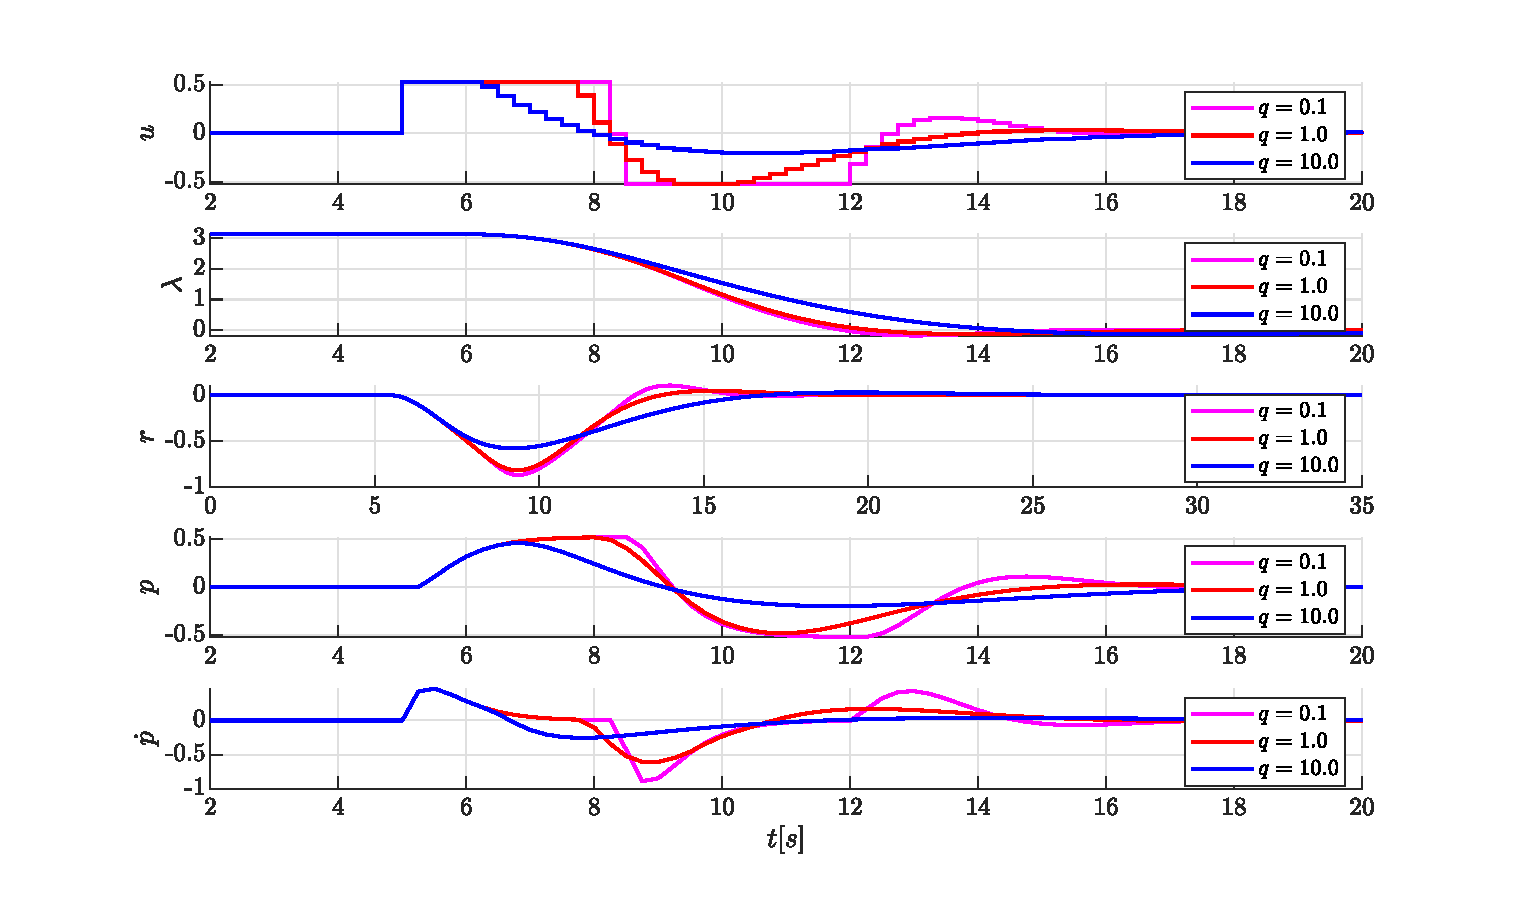
\includegraphics[width=\linewidth]{figures/lab2_optimal_u}
	\caption{Optimal trajectories for the manipulated variable and outputs with different values of $q$.}
	\label{fig:lab2_optimalu}
\end{figure}

\Cref{fig:lab2_optimalu} also shows how the constraints work in practice. Studying the plot of $ u $, we can see that no matter how low $ q $ is, the input never goes beyond the specified range of $ \pm\frac{30}{180} \pi $.

\subsection{The objective function}
\textit{Furthermore, discuss the objective function (15) (in the lab assignment text) in particular the term $(\lambda_i-\lambda_f )^2$. For instance, could any unwanted effects arise from steering the helicopter to $\lambda =\lambda_f$ with this objective function?}

From the forum: Here are some questions that will help you figure out what is asked for:
What will happen when you have some elements that are very large compared to others in a quadratic objective function? Which consequence(s) does this have for the setup in the lab? What is the impact of the length of the control horizon (imagine that the step length, h, is fixed)?

\clearpage
\subsection{Experimental results}\label{kap:task_10_2_experimental_results}
\textit{Printouts of data from relevant experiments (plots).
Discussion and analysis of the results.
Answer 10.2.2.7 here.}

\begin{figure}[h]
	\includegraphics[width=\linewidth]{figures/LAB2_plot_1.png}
	\caption{Results of LAB2}
	\label{fig:LAB2_plot_1}
\end{figure}

As \cref{fig:LAB2_plot_1} clearly shows the control sequence did not yield the desired travel-response. This is expected, as there is no feedback - any small variations will move the response from the planned one. In this case the variations are quite large, particularly the offset from what the encoder measures as $0$ pitch as opposed to what the real-world $0$ pitch is. This difference makes the helicopter travel while it keeps $0$-pitch.

The response shows a major travel-offset from the generated sequence, this is primarily because of the offset described above. The pitch-response is however quite close to the optimal trajectory - this is expected as there is not the same level of offset as in travel.

\subsection{MATLAB and Simulink}
\subsubsection{MATLAB}
\lstinputlisting[caption= {MATALB code for lab 2}, label={lst:lab2_matlab}]{code/lab2.m}
\subsubsection{Simulink}
\begin{figure}[h]
	\centering
	\includegraphics[width=\linewidth]{code/lab2_simulink}
	\caption{Simulink diagram used in lab 2.}
	\label{fig:lab2_simulink}
\end{figure}
\todo[inline]{Need a much better image of this.}
\end{document}